%% =======================================================
%% Actividad 8: Implementación de modelos predictivos con incertidumbre
%%
%% Compilar desde actividades/: ./compilar.sh act08
%% Las figuras de img/ se generan con: python act08.py
%% =======================================================

%% ---- CONFIGURACIÓN ------------------------

\documentclass[11pt,letterpaper]{article}

\usepackage[indice]{tecnm}
\usepackage[T1]{fontenc}
\usepackage{amsmath}
\usepackage{xcolor}
\usepackage{needspace}
\usepackage[most]{tcolorbox} % Carga tcolorbox con soporte para listings y saltos de página
\tcbuselibrary{listings, skins, breakable}
\setlength{\emergencystretch}{3em} % Evita líneas desbordadas por palabras en \texttt

% Paleta de colores (estilo GitHub Light / VS Code)
\definecolor{codebg}{HTML}{F8F9FA}       % Fondo del código
\definecolor{codehead}{HTML}{E9ECEF}     % Fondo de la barra de título
\definecolor{codeborder}{HTML}{CED4DA}   % Borde de la tarjeta
\definecolor{codetitle}{HTML}{212529}    % Texto del título
\definecolor{codekw}{HTML}{0550AE}       % Palabras clave (import, def, for...)
\definecolor{codefunc}{HTML}{8250DF}     % Funciones y métodos (describe, groupby...)
\definecolor{codestr}{HTML}{0A3069}      % Strings
\definecolor{codecomm}{HTML}{6E7781}     % Comentarios
\definecolor{codenum}{HTML}{8C959F}      % Números de línea
\definecolor{codeid}{HTML}{24292F}       % Texto general

% Configuración base de listings
\lstdefinestyle{pythonestilo}{
  language=Python,
  basicstyle=\ttfamily\footnotesize\color{codeid},
  keywordstyle=\color{codekw}\bfseries,
  keywordstyle=[2]\color{codefunc}, % Estilo secundario para métodos de datos
  stringstyle=\color{teal!80!black},
  commentstyle=\color{codecomm}\itshape,
  morekeywords={as, True, False, None, with, yield, lambda},
  morekeywords=[2]{print, len, sum, max, DataFrame, Series, value_counts, reindex, mean, std, var, randint, normal, seed, cumsum, predict_proba, predict, fit, train_test_split, make_blobs, GaussianNB, chisquare, pdf, cdf, hist, bar, plot, axhline, axvline, fill_between, subplots, figure, concat, nunique, load_iris, diff, sort, unique},
  numbers=left,
  numberstyle=\tiny\ttfamily\color{codenum},
  stepnumber=1,
  numbersep=10pt,
  showstringspaces=false,
  morestring=[b]{"""},
  tabsize=4,
  breaklines=true,
  breakatwhitespace=true,
  columns=flexible,
  keepspaces=true,
  literate=
    {á}{{\'a}}1 {é}{{\'e}}1 {í}{{\'i}}1 {ó}{{\'o}}1 {ú}{{\'u}}1
    {Á}{{\'A}}1 {É}{{\'E}}1 {Í}{{\'I}}1 {Ó}{{\'O}}1 {Ú}{{\'U}}1
    {ñ}{{\~n}}1 {Ñ}{{\~N}}1 {¿}{{?`}}1 {¡}{{!`}}1 {°}{{$^\circ$}}1
}

% Definición del entorno personalizado \begin{codigo}{Título}{etiqueta}
% \newtcblisting[auto counter, number within=section]{codigo}[2][]{
\newtcblisting[auto counter]{codigo}[2][]{
  listing only,
  breakable,                    % Permite que el bloque se divida si pasa de página
  enhanced,
  colback=codebg,
  colframe=codeborder,
  colbacktitle=codehead,
  coltitle=codetitle,
  fonttitle=\bfseries\small\sffamily,
  boxrule=0.6pt,
  arc=4pt,                      % Bordes redondeados
  left=20pt,                    % Espacio izquierdo para los números de línea
  right=8pt,
  top=6pt,
  bottom=6pt,
  toptitle=4pt,
  bottomtitle=4pt,
  before skip=12pt,
  after skip=12pt,
  listing options={style=pythonestilo},
  title={Código \thetcbcounter: #2},
  #1
}

% Paleta para salida de consola (estilo terminal limpia)
\definecolor{termbg}{HTML}{212529}      % Fondo oscuro tipo terminal
\definecolor{termhead}{HTML}{343A40}    % Barra superior
\definecolor{termtext}{HTML}{F8F9FA}    % Texto claro de alta legibilidad
\definecolor{termborder}{HTML}{495057}  % Borde

% Entorno \begin{consola}[label=out:iris]{Título}
\newtcblisting[auto counter]{consola}[2][]{
  listing only,
  breakable,
  colback=termbg,
  colframe=termborder,
  colbacktitle=termhead,
  coltitle=termtext,
  colupper=termtext,
  fonttitle=\bfseries\small\sffamily,
  boxrule=0.6pt,
  arc=4pt,
  left=8pt,
  right=8pt,
  top=6pt,
  bottom=6pt,
  toptitle=4pt,
  bottomtitle=4pt,
  before skip=12pt,
  after skip=12pt,
  listing options={
    basicstyle=\ttfamily\scriptsize\color{termtext}, % \scriptsize evita que las tablas de Pandas se partan de línea
    breaklines=true,
    columns=fixed,        % Mantiene alineadas las columnas de Pandas
    keepspaces=true,
    showstringspaces=false,
    literate=
      {á}{{\'a}}1 {é}{{\'e}}1 {í}{{\'i}}1 {ó}{{\'o}}1 {ú}{{\'u}}1
      {Á}{{\'A}}1 {É}{{\'E}}1 {Í}{{\'I}}1 {Ó}{{\'O}}1 {Ú}{{\'U}}1
      {ñ}{{\~n}}1 {Ñ}{{\~N}}1 {°}{{$^\circ$}}1
  },
  title={Salida \thetcbcounter: #2},
  #1
}

%% ---- DATOS DE LA MATERIA ------------------------

\materia{Modelos Estadísticos para el Aprendizaje \\ Automático y Ciencia de Datos}
\actividad{Tema 2.1
Variables Aleatorias: Tipos, Ejemplos, Representación Computacional \\ Actividad 8 - Implementación de Modelos Predictivos con Incertidumbre}

\profesor{Dr. José Ismael Ojeda Campaña}
%\fecha{15 de octubre de 2026}    % opcional; por defecto es la fecha de hoy

\begin{document}
\portada
\indicegeneral

%% ---- CONTENIDO ---------------------------------

\section{Introducción}

Un modelo de clasificación no solo debe decir a qué clase pertenece una observación, sino también qué tan seguro está de esa respuesta. En el aprendizaje automático los datos son inciertos por el ruido de las mediciones, por la cobertura incompleta del dominio y por la imperfección de los propios modelos, y las variables aleatorias permiten cuantificar esa incertidumbre \parencite{tecnm2026_documento_fuente,brownlee2020}. Por eso muchos clasificadores entregan probabilidades y no únicamente clases.

En este documento se construye un clasificador Naive Bayes Gaussiano para el conjunto de datos Iris \parencite{fisher1936}, dividido en 70\,\% para entrenamiento y 30\,\% para prueba, y se usan sus probabilidades predichas para evaluar la incertidumbre de cada predicción. Se analizan los casos en que el modelo duda entre dos especies, se visualiza la distribución de las probabilidades con histogramas y se mide cómo el ruido en las mediciones degrada las predicciones. Finalmente, se discute cómo cuantificar la incertidumbre mejora la interpretación del modelo y qué limitaciones tiene.

\section{Marco conceptual}

\subsection{Incertidumbre en el aprendizaje automático}

El aprendizaje automático trata de desarrollar modelos predictivos a partir de datos inciertos. El documento fuente identifica tres orígenes de la incertidumbre \parencite{tecnm2026_documento_fuente}:

\begin{itemize}
    \item \textbf{Ruido en las observaciones:} errores de medición y ruido aleatorio.
    \item \textbf{Cobertura incompleta del dominio:} no es posible observar todos los casos.
    \item \textbf{Modelos imperfectos:} todos los modelos cometen errores.
\end{itemize}

La probabilidad y las variables aleatorias permiten cuantificar y gestionar esta incertidumbre. La salida de un modelo predictivo puede verse como una variable aleatoria discreta sobre las clases posibles, y predecir probabilidades, y no solo clases, permite evaluar la incertidumbre de cada predicción \parencite{tecnm2026_documento_fuente,brownlee2020}.

\subsection{Naive Bayes}

Un clasificador probabilístico estima la probabilidad condicional de cada clase $y_i$ dadas las características observadas $x_1, \ldots, x_n$. Calcular directamente $P(x_1, \ldots, x_n \mid y_i)$ no es factible salvo con un número extraordinariamente grande de ejemplos, por lo que Naive Bayes simplifica el cálculo suponiendo que cada variable de entrada es independiente de las demás dada la clase \parencite{tecnm2026_documento_fuente,brownlee2020}:
\begin{equation}
    P(y_i \mid x_1, \ldots, x_n) \propto P(x_1 \mid y_i) \times P(x_2 \mid y_i) \times \cdots \times P(x_n \mid y_i) \times P(y_i).
\end{equation}
Se omite el denominador porque es una constante que solo normaliza el resultado. La clase con la puntuación proporcional más alta se elige como clasificación, regla que se conoce como decisión máxima a posteriori (MAP) \parencite{tecnm2026_documento_fuente}. Dividir las puntuaciones entre su suma las convierte en las probabilidades que entrega \texttt{predict\_proba()}.

La probabilidad a priori $P(y_i)$ se estima como la fracción de ejemplos de entrenamiento con esa clase. Para $P(x_j \mid y_i)$ se elige una distribución según el tipo de variable: multinomial para variables categóricas, binomial para variables binarias y gaussiana para variables numéricas, lo que da lugar a las variantes Multinomial, Binomial y Gaussian Naive Bayes. Con $K$ clases y $n$ variables hay que manejar $K \times n$ distribuciones \parencite{tecnm2026_documento_fuente}. En la variante Gaussiana, para cada clase y cada característica se estiman la media $\mu$ y la desviación estándar $\sigma$ de una distribución normal con los datos de entrenamiento.

\subsection{Medidas de incertidumbre de una predicción}

A partir del vector de probabilidades $\mathbf{p} = (p_1, \ldots, p_K)$ que produce el modelo para una observación se pueden calcular varias medidas de su incertidumbre:

\begin{itemize}
    \item \textbf{Confianza:} la probabilidad de la clase predicha, $\max_k p_k$. Con tres clases, el mínimo posible es $1/3$.
    \item \textbf{Margen:} la diferencia entre las dos probabilidades más altas. Un margen cercano a 0 indica que el modelo duda entre dos clases; con dos clases equivale a probabilidades cercanas a 0.5.
    \item \textbf{Entropía:} $H(\mathbf{p}) = -\sum_k p_k \log_2 p_k$, que vale 0 cuando el modelo está completamente seguro y $\log_2 K$ cuando todas las clases son igualmente probables \parencite{brownlee2020}.
\end{itemize}

\subsection{Ruido y limitaciones del modelo}

El ruido de medición hace que los valores observados se desvíen de los valores verdaderos de la característica. Un modelo entrenado con mediciones limpias puede degradarse al recibir observaciones ruidosas, y no necesariamente avisa de ello: sus probabilidades solo son confiables si los supuestos del modelo se cumplen \parencite{tecnm2026_documento_fuente,brownlee2020}. En Naive Bayes, el supuesto principal es la independencia condicional de las características, que en datos reales rara vez se cumple exactamente.

\section{Descripción de la actividad}

\textbf{Objetivo:} Aplicar variables aleatorias en la construcción de un modelo de clasificación simple, evaluando la incertidumbre en las predicciones \parencite{tecnm2026_documento_fuente}.

La actividad consta de cuatro tareas:

\begin{description}
    \item[a) Preparación de datos.] Cargar el dataset Iris con \texttt{sklearn.datasets.load\_iris} y dividirlo en entrenamiento (70\,\%) y prueba (30\,\%).
    \item[b) Modelado con Naive Bayes.] Entrenar un clasificador \texttt{GaussianNB} con los datos de entrenamiento y realizar predicciones probabilísticas sobre el conjunto de prueba.
    \item[c) Evaluación de incertidumbre.] Analizar los casos donde el modelo asigna probabilidades cercanas a 0.5 entre clases y visualizar la distribución de las probabilidades predichas con histogramas.
    \item[d) Interpretación de resultados.] Discutir cómo la cuantificación de la incertidumbre mejora la interpretación del modelo e identificar limitaciones relacionadas con el ruido en los datos.
\end{description}

\section{Desarrollo}

El script usa \texttt{numpy}, \texttt{pandas}, \texttt{matplotlib} y \texttt{scikit-learn}. Las particiones y los experimentos de ruido usan semillas fijas para que los resultados sean reproducibles, y las figuras se guardan como imágenes PNG en la carpeta \texttt{img/}. El Código~\ref{cod:comun} contiene las importaciones y la función auxiliar \texttt{guardar()}, que además muestra las figuras en pantalla cuando el código se ejecuta en un cuaderno. El cuaderno interactivo puede consultarse en Google Colab:

\begin{center}
    \url{https://colab.research.google.com/drive/1BOqun-mlGIBCZC1HIuHZ9NvDCAfb_roL?usp=sharing}
\end{center}

\begin{codigo}[label=cod:comun]{Importaciones y función auxiliar}
import os

import matplotlib

# En Colab o Jupyter no existe __file__; ahí las figuras también se muestran en pantalla
EN_NOTEBOOK = '__file__' not in globals()
if not EN_NOTEBOOK:
    matplotlib.use('Agg')  # Como script, genera las figuras como archivos PNG sin abrir ventanas

import matplotlib.pyplot as plt
import numpy as np
import pandas as pd
from sklearn.datasets import load_iris, make_blobs
from sklearn.metrics import accuracy_score, confusion_matrix
from sklearn.model_selection import train_test_split
from sklearn.naive_bayes import GaussianNB

pd.set_option('display.width', 100)

# Carpeta donde se guardan las figuras que se incluyen en el reporte
BASE = os.getcwd() if EN_NOTEBOOK else os.path.dirname(os.path.abspath(__file__))
CARPETA_IMG = os.path.join(BASE, 'img')
os.makedirs(CARPETA_IMG, exist_ok=True)


def guardar(nombre):
    """Guarda la figura actual en la carpeta img/ y la muestra si se ejecuta en un notebook."""
    plt.tight_layout()
    plt.savefig(os.path.join(CARPETA_IMG, nombre), dpi=150)
    if EN_NOTEBOOK:
        plt.show()
    plt.close()
\end{codigo}

\subsection{Código base del documento}

Antes de las tareas se ejecutó el ejemplo del documento fuente: se generan 100 puntos de dos clases con \texttt{make\_blobs}, se entrena un \texttt{GaussianNB} con todos ellos y se predice la primera muestra. \texttt{predict\_proba()} devuelve una probabilidad por clase y \texttt{predict()} devuelve la clase con la probabilidad más alta \parencite{tecnm2026_documento_fuente}.

\begin{codigo}[label=cod:base]{Código base: Naive Bayes con datos sintéticos}
# Generar un conjunto de datos sintético para clasificación (2 clases, 2 características)
X, y = make_blobs(n_samples=100, centers=2, n_features=2, random_state=1)

# Definir el modelo Naive Bayes Gaussiano
modelo = GaussianNB()

# Ajustar (entrenar) el modelo con los datos
modelo.fit(X, y)

# Seleccionar una muestra para predecir
Xmuestra, ymuestra = [X[0]], y[0]

# Realizar una predicción probabilística
probabilidades_predichas = modelo.predict_proba(Xmuestra)
print('Probabilidades predichas:', probabilidades_predichas)

# Realizar una predicción de clase
clase_predicha = modelo.predict(Xmuestra)
print('Clase predicha:', clase_predicha)
print('Clase real:', ymuestra)
\end{codigo}

\subsection{Tarea a: Preparación de datos}

El Iris Dataset tiene 150 flores de tres especies (setosa, versicolor y virginica) con cuatro medidas en centímetros: longitud y ancho del sépalo y del pétalo. La división se hizo con \texttt{train\_test\_split(test\_size=0.3)}, lo que deja 105 flores para entrenar y 45 para probar. Se usó \texttt{stratify=y} para que cada especie quede en la misma proporción en ambos conjuntos (15 flores de cada una en la prueba); sin estratificar, una especie podría quedar sobrerrepresentada por azar.

\begin{codigo}[label=cod:a]{Tarea a: Iris dividido en entrenamiento y prueba}
iris = load_iris()
CLASES = iris.target_names
X, y = iris.data, iris.target

# stratify conserva la misma proporción de especies en ambos conjuntos
X_ent, X_pru, y_ent, y_pru = train_test_split(X, y, test_size=0.3, random_state=42,
                                              stratify=y)

print("\n=== a) Preparación de datos ===")
print(f"Total: {len(X)} flores, {X.shape[1]} características")
print(f"Entrenamiento: {len(X_ent)} flores   Prueba: {len(X_pru)} flores")
print("Flores por especie en prueba:",
      {str(c): int(n) for c, n in zip(CLASES, np.bincount(y_pru))})
\end{codigo}

\subsection{Tarea b: Modelado con Naive Bayes}

\texttt{GaussianNB} estima, con las 105 flores de entrenamiento, una media y una varianza por cada característica y especie (12 distribuciones normales) y la probabilidad a priori de cada especie. \texttt{predict\_proba()} devuelve para cada flor de prueba una fila con tres probabilidades que suman 1. Se armó un \texttt{DataFrame} con esas probabilidades, la especie real, la predicha y si fue correcta, y se calculó la exactitud y la matriz de confusión. Como extensión, se comparó la exactitud con la de la partición del documento fuente (que no estratifica) y con la de 200 particiones aleatorias, para saber si el resultado depende de qué flores caen en la prueba.

\begin{codigo}[label=cod:b]{Tarea b: entrenamiento y predicciones probabilísticas}
modelo = GaussianNB()
modelo.fit(X_ent, y_ent)

# Predicción probabilística: una probabilidad por especie para cada flor de prueba
probabilidades = modelo.predict_proba(X_pru)
predicciones = modelo.predict(X_pru)

resultados = pd.DataFrame(probabilidades, columns=[f'P({c})' for c in CLASES])
resultados['Real'] = CLASES[y_pru]
resultados['Predicha'] = CLASES[predicciones]
resultados['Correcta'] = predicciones == y_pru

print("\n=== b) Modelado con GaussianNB ===")
print("Media de cada característica por especie (parámetro mu de cada normal):")
print(pd.DataFrame(modelo.theta_, index=CLASES,
                   columns=['sep_len', 'sep_wid', 'pet_len', 'pet_wid']).round(2))
print("\nPrimeras 8 predicciones del conjunto de prueba:")
print(resultados.head(8).round(4).to_string())
print(f"\nExactitud en prueba: {accuracy_score(y_pru, predicciones):.4f} "
      f"({(predicciones == y_pru).sum()} de {len(y_pru)})")
print("Matriz de confusión (filas = real, columnas = predicha):")
print(pd.DataFrame(confusion_matrix(y_pru, predicciones), index=CLASES, columns=CLASES))

# La exactitud depende de qué flores caen en la prueba: partición del documento fuente
# (random_state=42, sin estratificar) y variación en 200 particiones aleatorias 70/30
X_ent_doc, X_pru_doc, y_ent_doc, y_pru_doc = train_test_split(X, y, test_size=0.3,
                                                              random_state=42)
exactitud_doc = accuracy_score(y_pru_doc, GaussianNB().fit(X_ent_doc, y_ent_doc)
                               .predict(X_pru_doc))
exactitudes_particiones = []
for semilla in range(200):
    a, b, c, d = train_test_split(X, y, test_size=0.3, random_state=semilla, stratify=y)
    exactitudes_particiones.append(accuracy_score(d, GaussianNB().fit(a, c).predict(b)))
exactitudes_particiones = np.array(exactitudes_particiones)

print(f"\nExactitud con la partición del documento fuente (sin estratificar): "
      f"{exactitud_doc:.4f}")
print(f"Exactitud en 200 particiones estratificadas: media {exactitudes_particiones.mean():.4f}, "
      f"desv. estándar {exactitudes_particiones.std(ddof=1):.4f}")
print(f"  mín. {exactitudes_particiones.min():.4f}, máx. {exactitudes_particiones.max():.4f}")
\end{codigo}

\subsection{Tarea c: Evaluación de la incertidumbre}

La función \texttt{medidas\_incertidumbre()} calcula para cada flor la confianza, el margen entre las dos especies más probables y la entropía. Como el problema tiene tres clases, un caso ambiguo se definió como aquel en que las dos especies más probables están cerca una de la otra, es decir, con margen menor que 0.5; el caso de dos clases con probabilidades de 0.5 y 0.5 es el extremo de esta definición. También se calculó la exactitud en cada nivel de confianza para verificar si la confianza del modelo es informativa, se listaron las predicciones incorrectas y se dibujaron los histogramas de las probabilidades predichas y un mapa de las flores coloreadas por su confianza.

\begin{codigo}[label=cod:c]{Tarea c: incertidumbre de las predicciones}
def medidas_incertidumbre(probabilidades):
    """Confianza, margen entre las dos clases más probables y entropía de cada predicción."""
    ordenadas = np.sort(probabilidades, axis=1)
    confianza = ordenadas[:, -1]
    margen = ordenadas[:, -1] - ordenadas[:, -2]
    p = np.clip(probabilidades, 1e-12, 1)
    entropia = -(p * np.log2(p)).sum(axis=1)
    return confianza, margen, entropia


confianza, margen, entropia = medidas_incertidumbre(probabilidades)
resultados['Confianza'] = confianza
resultados['Margen'] = margen
resultados['Entropía'] = entropia

# Casos ambiguos: las dos especies más probables están cerca de 0.5 cada una
UMBRAL_MARGEN = 0.5
ambiguos = resultados[resultados['Margen'] < UMBRAL_MARGEN]

print("\n=== c) Evaluación de la incertidumbre ===")
print(f"Confianza media: {confianza.mean():.4f}   mínima: {confianza.min():.4f}")
print(f"Predicciones con confianza > 0.99: {(confianza > 0.99).sum()} de {len(confianza)}")
print(f"Casos ambiguos (margen < {UMBRAL_MARGEN}): {len(ambiguos)}")
print(ambiguos[['P(setosa)', 'P(versicolor)', 'P(virginica)', 'Real', 'Predicha', 'Margen']]
      .round(4).to_string())

# Exactitud según el nivel de confianza
grupos = pd.cut(resultados['Confianza'], bins=[0, 0.9, 0.99, 1.0],
                labels=['< 0.90', '0.90-0.99', '> 0.99'])
por_confianza = resultados.groupby(grupos, observed=False)['Correcta'].agg(['count', 'mean'])
por_confianza.columns = ['Flores', 'Exactitud']
print("\nExactitud por nivel de confianza:")
print(por_confianza.round(3))

errores = resultados[~resultados['Correcta']]
print(f"\nPredicciones incorrectas: {len(errores)}")
print(errores[['Real', 'Predicha', 'Confianza', 'Margen']].round(4).to_string())

# Histogramas de las probabilidades predichas
fig, axes = plt.subplots(1, 4, figsize=(15, 3.8))
for ax, (i, clase) in zip(axes, enumerate(CLASES)):
    ax.hist(probabilidades[:, i], bins=np.linspace(0, 1, 21), color=f'C{i}', edgecolor='black')
    ax.set_title(f'P({clase})')
    ax.set_xlabel('Probabilidad predicha')
    ax.set_ylabel('Flores')
axes[3].hist(confianza, bins=np.linspace(0, 1, 21), color='gray', edgecolor='black')
axes[3].axvline(0.5, color='red', linestyle='--', label='0.5')
axes[3].set_title('Confianza (probabilidad máxima)')
axes[3].set_xlabel('Probabilidad máxima')
axes[3].legend()
guardar('c_histogramas_probabilidades.png')

# Mapa de las flores de prueba según la confianza del modelo
plt.figure(figsize=(7.5, 5))
puntos = plt.scatter(X_pru[:, 2], X_pru[:, 3], c=confianza, cmap='viridis', vmin=0.5, vmax=1,
                     s=60, edgecolor='black')
plt.scatter(X_pru[margen < UMBRAL_MARGEN, 2], X_pru[margen < UMBRAL_MARGEN, 3], s=220,
            facecolors='none', edgecolors='red', linewidth=2, label='Caso ambiguo')
plt.scatter(X_pru[predicciones != y_pru, 2], X_pru[predicciones != y_pru, 3], marker='x',
            color='red', s=80, label='Predicción incorrecta')
plt.colorbar(puntos, label='Confianza')
plt.title('Flores de prueba coloreadas por la confianza del modelo')
plt.xlabel('Longitud del pétalo (cm)')
plt.ylabel('Ancho del pétalo (cm)')
plt.legend(loc='upper left')
guardar('c_confianza_petalos.png')
\end{codigo}

\subsection{Tarea d: Limitaciones del modelo y ruido en los datos}

Para estudiar el efecto del ruido se sumó ruido gaussiano $N(0, \sigma_r)$ a las cuatro medidas de las flores de prueba, como si fueran errores de medición, con $\sigma_r$ entre 0 y 1 cm; el modelo no se vuelve a entrenar. Como el ruido es aleatorio, cada nivel se repitió 50 veces y se promediaron la exactitud, la confianza media, la confianza media de las predicciones incorrectas y el porcentaje de casos ambiguos. Además, se calculó la correlación entre la longitud y el ancho del pétalo dentro de cada especie para revisar el supuesto de independencia de Naive Bayes.

\begin{codigo}[label=cod:d]{Tarea d: efecto del ruido y supuesto de independencia}
# Se agrega ruido gaussiano a las mediciones de prueba, como errores de medición
rng = np.random.default_rng(8)
NIVELES_RUIDO = [0.0, 0.1, 0.2, 0.3, 0.5, 0.75, 1.0]
REPETICIONES = 50

filas = []
for sd in NIVELES_RUIDO:
    exactitudes, confianzas, confianzas_error, ambiguos_pct = [], [], [], []
    for _ in range(REPETICIONES):
        X_ruido = X_pru + rng.normal(0, sd, X_pru.shape)
        prob = modelo.predict_proba(X_ruido)
        conf, marg, _ = medidas_incertidumbre(prob)
        exactitudes.append(accuracy_score(y_pru, prob.argmax(axis=1)))
        confianzas.append(conf.mean())
        incorrectas = prob.argmax(axis=1) != y_pru
        if incorrectas.any():
            confianzas_error.append(conf[incorrectas].mean())
        ambiguos_pct.append((marg < UMBRAL_MARGEN).mean() * 100)
    filas.append({'Ruido (cm)': sd, 'Exactitud': np.mean(exactitudes),
                  'Confianza media': np.mean(confianzas),
                  'Confianza en errores': np.mean(confianzas_error),
                  'Ambiguos (%)': np.mean(ambiguos_pct)})
ruido = pd.DataFrame(filas)

print("\n=== d) Efecto del ruido en las mediciones (promedio de 50 repeticiones) ===")
print(ruido.round(3).to_string(index=False))

# El supuesto "naive": las características son independientes dentro de cada especie
correlaciones = {clase: np.corrcoef(X_ent[y_ent == i][:, 2], X_ent[y_ent == i][:, 3])[0, 1]
                 for i, clase in enumerate(CLASES)}
print("\nCorrelación entre longitud y ancho del pétalo dentro de cada especie:")
print({str(c): round(float(r), 3) for c, r in correlaciones.items()})

plt.figure(figsize=(7.5, 4.5))
plt.plot(ruido['Ruido (cm)'], ruido['Exactitud'], 'o-', label='Exactitud')
plt.plot(ruido['Ruido (cm)'], ruido['Confianza media'], 's--', label='Confianza media')
plt.plot(ruido['Ruido (cm)'], ruido['Confianza en errores'], '^:',
         label='Confianza media en las predicciones incorrectas')
plt.xlabel('Desviación estándar del ruido agregado (cm)')
plt.ylabel('Proporción')
plt.ylim(0, 1.05)
plt.legend(loc='lower left')
plt.grid(linestyle='--', alpha=0.5)
plt.title('Efecto del ruido en las predicciones de GaussianNB')
guardar('d_ruido.png')

print(f"\nFiguras guardadas en {os.path.basename(CARPETA_IMG)}/")
\end{codigo}

\clearpage
\section{Resultados}

\subsection{Código base y tarea a: Preparación de datos}

\begin{consola}[label=out:a]{Ejecución de \texttt{act08.py}: código base y tarea a}
Probabilidades predichas: [[1.00000000e+00 5.52387327e-30]]
Clase predicha: [0]
Clase real: 0

=== a) Preparación de datos ===
Total: 150 flores, 4 características
Entrenamiento: 105 flores   Prueba: 45 flores
Flores por especie en prueba: {'setosa': 15, 'versicolor': 15, 'virginica': 15}
\end{consola}

En el ejemplo del documento, la primera muestra tiene probabilidad prácticamente 1 de la clase 0 y $5.5 \times 10^{-30}$ de la clase 1, por lo que el modelo la clasifica correctamente con total seguridad; es una predicción probabilística extrema porque los dos grupos de \texttt{make\_blobs} están bien separados. Con Iris, la división deja 105 flores de entrenamiento y 45 de prueba, 15 de cada especie.

\Needspace{34\baselineskip}
\subsection{Tarea b: Modelo y predicciones}

\begin{consola}[label=out:b]{Ejecución de \texttt{act08.py}: tarea b}
=== b) Modelado con GaussianNB ===
Media de cada característica por especie (parámetro mu de cada normal):
            sep_len  sep_wid  pet_len  pet_wid
setosa         4.99     3.43     1.49     0.24
versicolor     5.95     2.73     4.24     1.31
virginica      6.68     3.01     5.63     2.07

Primeras 8 predicciones del conjunto de prueba:
   P(setosa)  P(versicolor)  P(virginica)        Real    Predicha  Correcta
0        0.0         0.0000        1.0000   virginica   virginica      True
1        0.0         0.9955        0.0045  versicolor  versicolor      True
2        0.0         0.8472        0.1528   virginica  versicolor     False
3        0.0         0.6680        0.3320  versicolor  versicolor      True
4        0.0         0.1036        0.8964   virginica   virginica      True
5        0.0         0.0000        1.0000   virginica   virginica      True
6        0.0         1.0000        0.0000  versicolor  versicolor      True
7        0.0         1.0000        0.0000  versicolor  versicolor      True

Exactitud en prueba: 0.9111 (41 de 45)
Matriz de confusión (filas = real, columnas = predicha):
            setosa  versicolor  virginica
setosa          15           0          0
versicolor       0          14          1
virginica        0           3         12

Exactitud con la partición del documento fuente (sin estratificar): 0.9778
Exactitud en 200 particiones estratificadas: media 0.9528, desv. estándar 0.0277
  mín. 0.8667, máx. 1.0000
\end{consola}

\begin{itemize}
    \item \textbf{Parámetros aprendidos.} Las medias confirman las diferencias entre especies: la setosa tiene pétalos pequeños (longitud media 1.49 cm, ancho 0.24 cm), mientras que versicolor (4.24 y 1.31 cm) y virginica (5.63 y 2.07 cm) tienen pétalos más grandes y cercanos entre sí.
    \item \textbf{Predicciones.} Cada flor recibe una probabilidad por especie. En las primeras ocho filas, seis flores tienen una probabilidad predicha mayor que 0.89. La fila 2 es una virginica clasificada como versicolor con $P = 0.8472$: el modelo se equivoca, aunque no con total seguridad.
    \item \textbf{Exactitud.} El modelo acierta 41 de las 45 flores (91.1\,\%). Todas las setosa se clasifican bien; los cuatro errores se reparten entre versicolor y virginica: tres virginica se predicen como versicolor y una versicolor como virginica.
    \item \textbf{Dependencia de la partición.} Con la partición del documento fuente la exactitud es 97.8\,\%, pero en 200 particiones estratificadas la media es 95.3\,\% con desviación estándar de 2.8 puntos, y varía entre 86.7\,\% y 100\,\%. El 91.1\,\% obtenido aquí está por debajo del promedio: con solo 45 flores de prueba, un error más o menos cambia la exactitud en 2.2 puntos, por lo que un solo número es una estimación incierta del desempeño real del modelo.
\end{itemize}

\Needspace{28\baselineskip}
\subsection{Tarea c: Incertidumbre de las predicciones}

\begin{consola}[label=out:c]{Ejecución de \texttt{act08.py}: tarea c}
=== c) Evaluación de la incertidumbre ===
Confianza media: 0.9698   mínima: 0.6680
Predicciones con confianza > 0.99: 36 de 45
Casos ambiguos (margen < 0.5): 2
    P(setosa)  P(versicolor)  P(virginica)        Real    Predicha  Margen
3         0.0         0.6680        0.3320  versicolor  versicolor  0.3359
30        0.0         0.7108        0.2892   virginica  versicolor  0.4216

Exactitud por nivel de confianza:
           Flores  Exactitud
Confianza
< 0.90          6      0.667
0.90-0.99       3      0.333
> 0.99         36      1.000

Predicciones incorrectas: 4
          Real    Predicha  Confianza  Margen
2    virginica  versicolor     0.8472  0.6944
30   virginica  versicolor     0.7108  0.4216
39  versicolor   virginica     0.9236  0.8473
42   virginica  versicolor     0.9806  0.9613
\end{consola}

\begin{figure}[htbp]
\centering
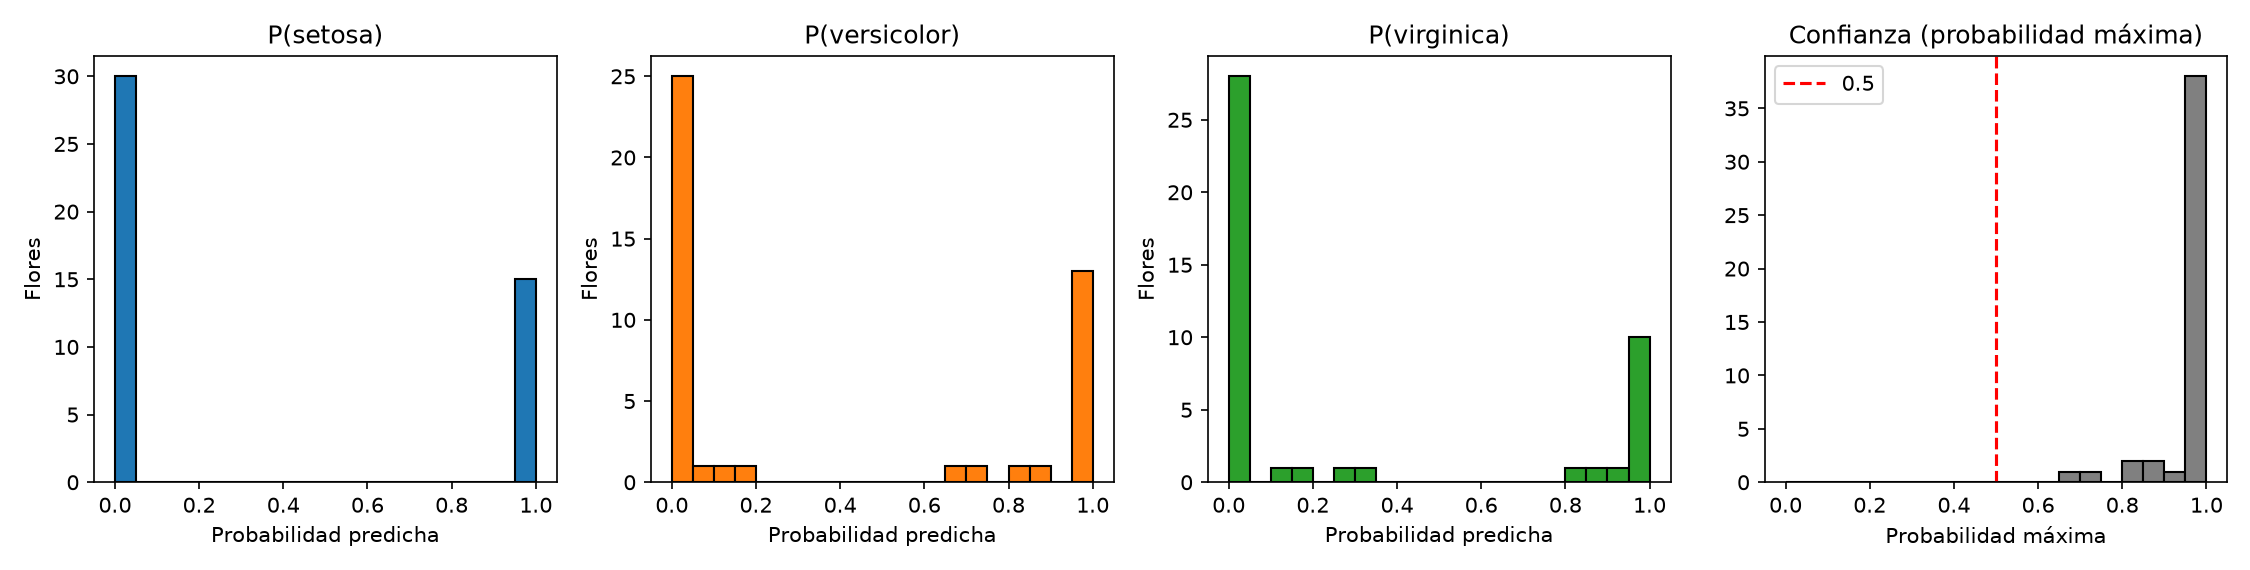
\includegraphics[width=\textwidth]{img/c_histogramas_probabilidades.png}
\caption{Histogramas de las probabilidades predichas para las 45 flores de prueba: una para cada especie y, a la derecha, la confianza (probabilidad máxima). La línea roja marca 0.5.}
\label{fig:histogramas}
\end{figure}

\begin{figure}[htbp]
\centering
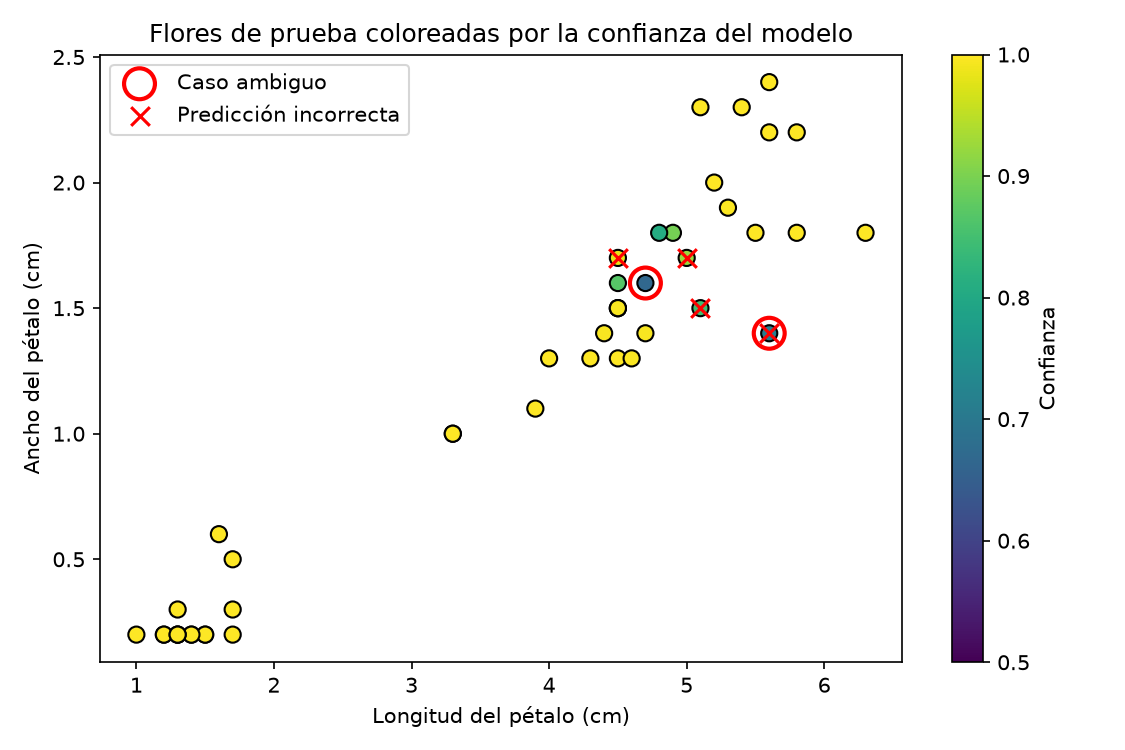
\includegraphics[width=0.78\textwidth]{img/c_confianza_petalos.png}
\caption{Flores de prueba según el tamaño de su pétalo, coloreadas por la confianza del modelo. Los círculos rojos marcan los casos ambiguos y las cruces rojas, las predicciones incorrectas.}
\label{fig:confianza}
\end{figure}

\begin{itemize}
    \item \textbf{Distribución de las probabilidades.} En la Figura~\ref{fig:histogramas} las probabilidades se concentran en los extremos: 0 o 1 para casi todas las flores. En el histograma de la confianza no hay ninguna flor por debajo de 0.5, ninguna con confianza menor que 0.66 y la mayoría está en el último intervalo. La confianza media es 0.970 y 36 de las 45 predicciones tienen confianza mayor que 0.99. Para la setosa, la probabilidad es prácticamente 0 o 1 en las 45 flores, lo que indica que esa especie está claramente separada de las otras dos.
    \item \textbf{Casos ambiguos.} Solo dos flores tienen margen menor que 0.5 (filas 3 y 30 de la Salida~\ref{out:c}): una versicolor con probabilidades 0.668 y 0.332, que el modelo acierta, y una virginica con 0.711 (versicolor) y 0.289 (virginica), que clasifica mal. En ningún caso las probabilidades se acercan a 0.5 de manera estricta; con datos tan bien separados, el modelo rara vez duda, y cuando lo hace es entre versicolor y virginica, nunca con la setosa. Ambas flores aparecen con colores oscuros (confianza menor) en la Figura~\ref{fig:confianza}, en la zona donde se traslapan las dos especies, con pétalos de 4.7 a 5.6 cm de longitud.
    \item \textbf{La confianza es informativa.} Las 36 predicciones con confianza mayor que 0.99 son todas correctas (exactitud de 100\,\%), mientras que las 6 predicciones con confianza menor que 0.90 solo aciertan en 66.7\,\% de los casos. El grupo intermedio (0.90 a 0.99) tiene solo 3 flores y una exactitud de 33.3\,\%, un tamaño demasiado pequeño para concluir algo. Aun así, las probabilidades permiten separar las predicciones confiables de las que conviene revisar.
    \item \textbf{La confianza no es infalible.} Una de las cuatro predicciones incorrectas tiene confianza 0.981 (fila 42, una virginica clasificada como versicolor): el modelo estaba casi seguro y se equivocó. Los otros tres errores tienen confianza de 0.71, 0.85 y 0.92. Una confianza alta reduce el riesgo de error, pero no lo elimina.
\end{itemize}

\Needspace{14\baselineskip}
\subsection{Tarea d: Efecto del ruido y supuesto de independencia}

\begin{consola}[label=out:d]{Ejecución de \texttt{act08.py}: tarea d}
=== d) Efecto del ruido en las mediciones (promedio de 50 repeticiones) ===
 Ruido (cm)  Exactitud  Confianza media  Confianza en errores  Ambiguos (%)
       0.00      0.911            0.970                 0.866         4.444
       0.10      0.906            0.965                 0.840         5.911
       0.20      0.894            0.966                 0.860         5.378
       0.30      0.858            0.970                 0.906         4.400
       0.50      0.783            0.969                 0.930         4.933
       0.75      0.678            0.968                 0.946         4.800
       1.00      0.596            0.971                 0.957         4.311

Correlación entre longitud y ancho del pétalo dentro de cada especie:
{'setosa': 0.255, 'versicolor': 0.737, 'virginica': 0.333}

Figuras guardadas en img/
\end{consola}

\begin{figure}[htbp]
\centering
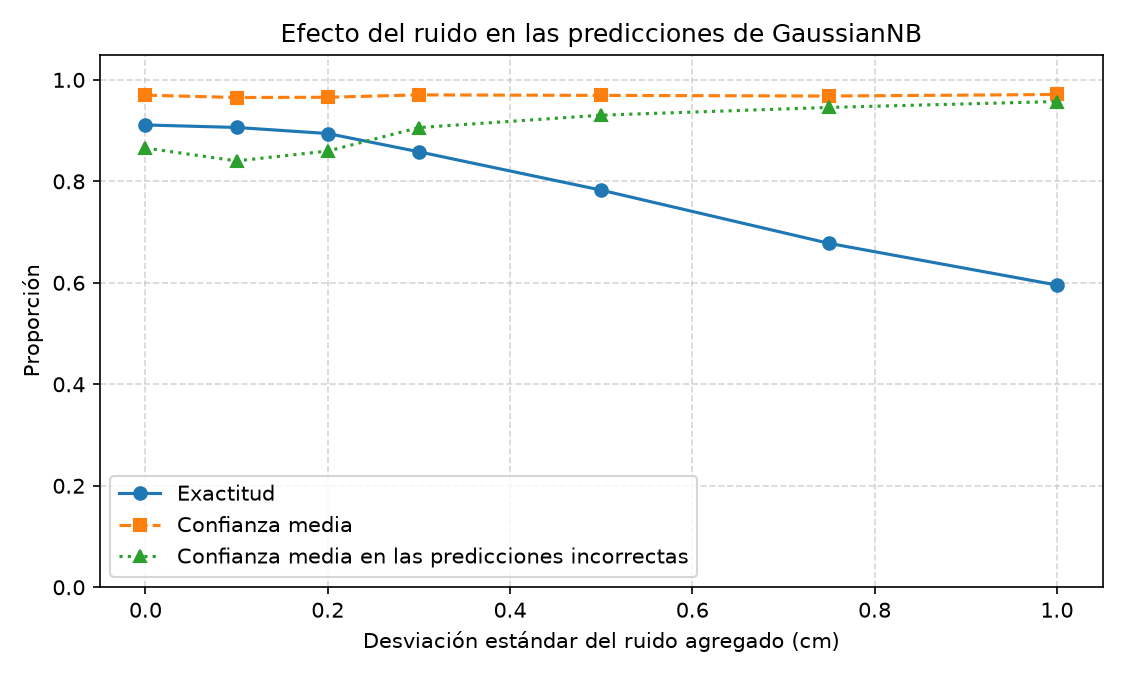
\includegraphics[width=0.78\textwidth]{img/d_ruido.png}
\caption{Exactitud, confianza media y confianza media de las predicciones incorrectas en función de la desviación estándar del ruido agregado a las mediciones de prueba (promedio de 50 repeticiones).}
\label{fig:ruido}
\end{figure}

\begin{itemize}
    \item \textbf{La exactitud cae con el ruido.} En la Figura~\ref{fig:ruido}, la exactitud baja de 0.911 sin ruido a 0.858 con $\sigma_r = 0.3$ cm, a 0.783 con 0.5 cm y a 0.596 con 1.0 cm, cerca de la mitad del camino entre el azar (0.33) y el desempeño sin ruido. La caída era previsible, porque las medias de versicolor y virginica difieren en alrededor de 1.4 cm en la longitud del pétalo y 0.8 cm en su ancho, y un ruido de esa magnitud borra la diferencia.
    \item \textbf{La confianza no refleja el ruido.} La confianza media permanece prácticamente constante, entre 0.965 y 0.971, mientras la exactitud pierde más de 30 puntos. Además, la confianza media de las predicciones incorrectas sube de 0.866 a 0.957: con más ruido, el modelo se equivoca más, pero con tanta seguridad como cuando acierta. El porcentaje de casos ambiguos tampoco crece (entre 4.3\,\% y 5.9\,\%). Esto ocurre porque una observación con ruido cae en las colas de las normales ajustadas, donde la razón entre las densidades de dos clases es muy grande y las probabilidades se saturan cerca de 0 y 1. El modelo trata los valores ruidosos como si fueran mediciones exactas.
    \item \textbf{Supuesto de independencia.} Dentro de cada especie, la longitud y el ancho del pétalo están correlacionados: 0.255 en setosa, 0.333 en virginica y 0.737 en versicolor. Naive Bayes supone que son independientes dada la especie, por lo que multiplica probabilidades que en realidad están relacionadas y cuenta dos veces parte de la misma información. Esto es una causa de que las probabilidades salgan más extremas de lo que justifican los datos.
\end{itemize}

\section{Conclusiones}

El clasificador \texttt{GaussianNB} separó las tres especies de Iris con una exactitud de 91.1\,\% en la partición de prueba, una estimación que resultó por debajo del promedio de 95.3\,\% de 200 particiones distintas. La salida del modelo como una distribución de probabilidad sobre las clases aporta más información que la clase predicha: la confianza distinguió las predicciones confiables (las 36 con confianza mayor que 0.99 fueron todas correctas) de las dudosas (solo 66.7\,\% de acierto con confianza menor que 0.90), y mostró que la incertidumbre se concentra entre versicolor y virginica, mientras que la setosa se clasifica siempre con seguridad. Esto permite decidir qué predicciones aceptar automáticamente y cuáles revisar.

Sin embargo, la cuantificación de la incertidumbre tiene límites que el análisis hizo visibles. Los casos con probabilidades cercanas a 0.5 son raros porque las probabilidades de Naive Bayes tienden a los extremos, y una predicción incorrecta puede tener confianza de 0.98. Más importante aún, cuando se agregó ruido a las mediciones la exactitud cayó de 0.91 a 0.60, pero la confianza media no se movió: el modelo no detecta que sus entradas son menos confiables. Por eso las probabilidades de Naive Bayes deben interpretarse como un orden entre predicciones, y no como la probabilidad real de acertar, sobre todo si los datos nuevos tienen más ruido que los de entrenamiento o las características no son independientes, como mostró la correlación de 0.74 entre la longitud y el ancho del pétalo en versicolor.

\referencias

\end{document}
